\section{Sistema Web}

El sitio web en el cual se implemento la solución presentada fue creado para una micro empresa de
ventas de video juegos, llamada Kurgan, ubicada en avenida Valparaíso 595 Local 9, Viña del Mar.
Su existencia es desde el año 2010 y su especialidad es la venta de consolas, video juegos y
accesorios y también se dedica a la venta de juegos coleccionables, en menor medida.

La investigación e implementación tuvo $2$ etapas. La primera de reconocimiento y obtención de
datos sin la implementación de la solución para crear un linea base del comportamiento de las visitas
y ventas por este medio. La segunda parte es luego de implementar las ideas propuestas tras la solución
propuestas y realizar una comparación para obtener conclusiones de la utilidad de \emph{gamification}
como una solución para mejorar las ventas de una micro o pequeña empresa.

\subsection{Datos pre implementación \emph{gamification}}

Esta primera etapa se dio inicio una vez implementada la base web, Wordpress + woocommerce, con
una base de productos, tanto videos juegos como accesorios. Tuvo una duración de 30 días, desde el 1
 al 30 de noviembre del año 2014, en los cuales se obtuvieron los siguientes datos importantes:

\begin{itemize}
\item Cantidad de visitas: 315 (visitas únicas).
\item Cantidad de lecturas: 445.
\item Cantidad de usuarios inscritos: 0.
\item Cantidad de ventas realizadas: 0.
\end{itemize}

Esta información ayudara a crear una linea base para poder comparar los resultados obtenidos una vez
implementada la idea de \emph{gamification} en el sitio web.

\subsection{Datos post implementación \emph{gamification}}

En esta etapa se implementaron los plugins para transformar el sistema web convencional de ventas
online a uno \emph{gamificado}. Estos plugins son los que implementan la acumulación de puntos,
logros y el encargado de realizar las referencias a los amigos.

Luego de obtener la base de comparación, esta nueva etapa tiene una duración de 30 días, desde
el 1 al 31 de diciembre del 2014. Los datos obtenidos son:

\begin{itemize}
\item Cantidad de visitas post implementación: 476 (visitas únicas).
\item Cantidad de lecturas: 641.
\item Cantidad de usuarios inscritos: 0.
\item Cantidad de ventas realizadas: 0.
\end{itemize}

\subsection{Comparación de datos}

Una vez obtenidos los datos estos entregaron información útil para llegar a conclusiones que serán
presentadas mas adelante.

Se puede observar que hubo un aumento en la cantidad de visitas y de lecturas. Esta comparación
ayuda a mostrar que se logro cumplir uno de los objetivos, atraer posibles clientes, de implementar
 \emph{gamification}. Este tema es importante debido a que si no se obtiene una mejora en la cantidad
de visitantes es bastante difícil establecer que la solución presentada ayuda a las micro o pequeña
empresa.

Por otro lado se puede observar que no se logro una mejora en lo que a nuevos usuarios registrados y
ventas se refiere. En la primera como en la segunda etapa, no hubo usuarios registrado y tampoco
una transacción, venta, realizada.
Luego de obtener estos datos durante $2$ meses se podría inferir que la utilización de {\GAM} no fue
efectiva durante este periodo, pero también pudo deberse a otros factores como la falta de difusión
de la tienda o que los beneficios propuestos no incentivaran a los clientes a comprar, bajos descuentos,
baja equivalencia de puntos o que los clientes suelen comprar por internet en lugares mas reconocidos.

Debido a que la información obtenida al reunir los datos por 2 meses no es concluyente para decir que
la utilización de {\GAM} no obtuvo los resultados esperados al ser implementada en una micro empresa se
diseño una encuesta con el objetivo de apoyar la utilización de {\GAM} en tiendas online.

A continuación se desarrolla y explica toda la encuesta realizada. Se analizan los datos obtenidos
con esta pregunta a pregunta.

\section{Encuesta}

Para complementar el presente trabajo, se realizó una encuesta con el objetivo de
conocer el conocimiento general de las personas con respecto a la existencia
de las técnicas asociadas a {\GAM}.
Por otro lado, se aprovechó la oportunidad para saber cuales son las preferencias
que tiene la gente a la hora de participar en sistemas que utilizan {\GAM},
siendo los más conocidos la acumulación de puntos en grandes empresas de retail,
para conseguir beneficios y recompensas.

Finalmente, podremos apreciar si la gente está dispuesta al uso de sistemas,
o ambientes de la vida cotidiana que utilicen características de {\GAM},
ya sean aplicadas a la educación, como al área laboral, lo cual demostrara
 si es que existen ciertas restricciones a la hora de aplicar
el principio expuesto en este trabajo, para el común de las personas
encuestadas.

\subsection{Metodología}

Para la validación de la encuesta se utilizó un intervalo de confianza de un 95\%, se espera que
este porcentaje de la población entregue respuestas verdaderas, con un error
muestral de 7.5\%, se estima que la variación de respuestas entre muestras poblacionales
 sera de cerca de este porcentaje además debido a la aleatoriedad de la población.
Dicho error muestral es más alto de lo normal, ya que la forma en la cual la encuesta fue difundida,
 nos entregará un universo más aleatorio. Se utilizaron las redes sociales las cuales
se conforman de un universo de personas con una gran homogeneidad.

Considerando nuestro intervalo de confianza y error muestral, se necesitan al menos 165
personas encuestadas para obtener una encuesta valida y que la muestra de población obtenida
se una muestra representativa de la población total.

Como se mencionó anteriormente, la encuesta fue difundida vía redes sociales,
y fue realizada utilizando la plataforma Google Form para un fácil análisis y almacenamiento
 de todas las respuestas.

La encuesta fue respondida por 180 personas, y los resultados obtenidos son descritos y
analizados a continuación.

\subsection{Datos e información}

De un universo de 180 personas encuestadas, el $71\%$ son hombres y el $29\%$ restante son mujeres.
Los rangos de edades de los encuestados van desde los 18 a 32 años, estando el $99\%$ de las personas
dentro de este rango.

Analizando la pregunta numero 3, ¿está al tanto de lo que es {\GAM}/Ludificación?, se obtiene que
 un $56\%$ de los encuestados ya tiene algún conocimiento sobre {\GAM}, mostrado en el gráfico~\ref{fig:chart5.1}.
Esta información es relevante al momento de implementar una solución gamificada.
Teniendo en cuenta que un gran porcentaje de la población de muestra es joven se puede infiere
que es la población con una capacidad mayor de aceptar el concepto de {\GAM} al ser implementado
como solución, en este caso en el contexto de ventas on-line.

\begin{figure}[!htb]
  \centering
  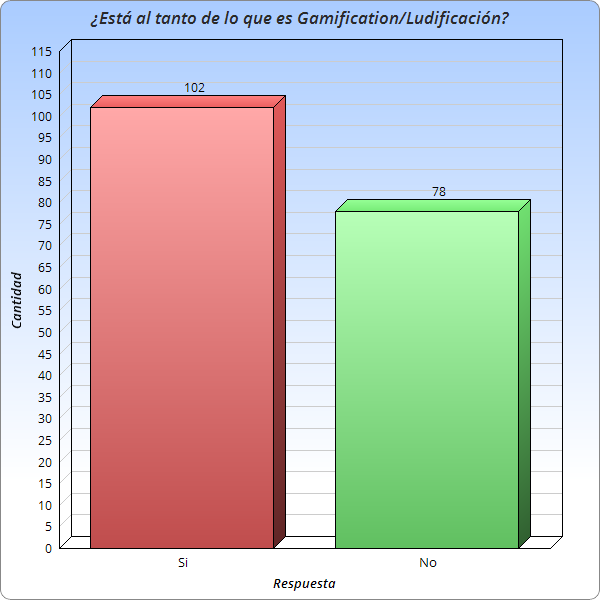
\includegraphics[width=0.6\textwidth]{images/Graficos/graf_5_1.png}
  \caption[chart5.1]{Respuesta a pregunta $3$, conocimiento de {\GAM}.}
  \label{fig:chart5.1}
  %\url{http://www.chartgo.com/get.do?id=69b1dc7d4e}
\end{figure}

La siguiente pregunta, ¿usted acumula puntos de grandes empresas? , fue creada con el motivo de
reforzarle al usuario una forma de {\GAM} con la cual se relaciona frecuentemente y así darle
a entender de mejor forma el concepto. En esta se obtiene un resultado similar al obtenido en
la pregunta anterior, donde un $56\%$ contesta positivamente. Con esta respuesta se ratifica que existe
algún conocimiento sobre {\GAM} por parte mas de la mitad de los encuestados, además se demuestra que
han interactuado con ella de alguna forma.

\begin{figure}[!htb]
  \centering
  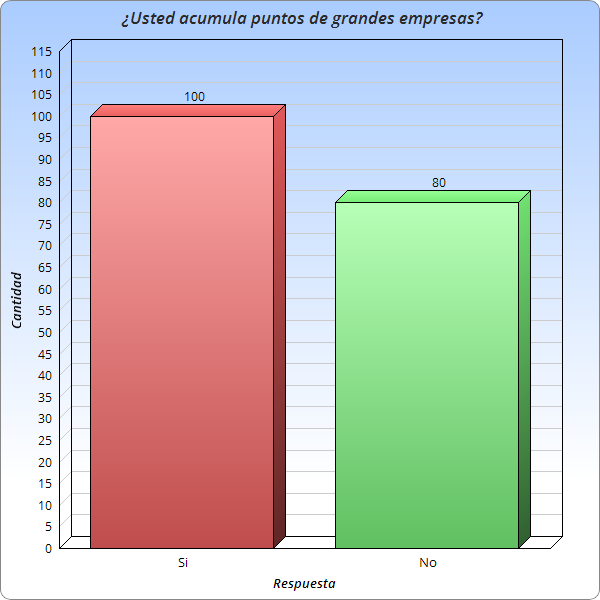
\includegraphics[width=0.6\textwidth]{images/Graficos/graf_5_2.png}
  \caption[chart5.2]{Respuesta a pregunta $4$, acumulación de puntos.}
  \label{fig:chart5.2}
  %\url{http://www.chartgo.com/get.do?id=69b1dc7d4e}
\end{figure}

Las preguntas $5$ y $6$ son exclusivas para las personas que respondieron positivamente la
pregunta anterior, numero $4$.Estas preguntas no son obligatorias por lo cual la muestra poblacional
es menor a la obtenida en la encuesta, ambas tienen universos diferentes.
En la primera existen $92$ encuestados que constituyen el $100\%$. Esta pregunta tiene como objetivo
conocer si los encuestados están en conocimiento de los beneficios entregados por las empresas.
Con $69$ personas contestando positivamente, equivalente a $75\%$, se puede apreciar que los
encuestados tienen conocimientos del fin detrás de la acumulación de puntos, y es esto lo que
crea el motivo de volver y seguir comprando en una tienda on-line o presencial.

La siguiente pregunta tiene un universo de $101$ personas, del cual un $78\%$ contesto de forma positiva.
Con esto se remarca que los encuestados están en conocimiento de toda la información necesaria
para motivarlos a seguir y conquistar su meta.

\begin{figure}[!htb]
  \centering
  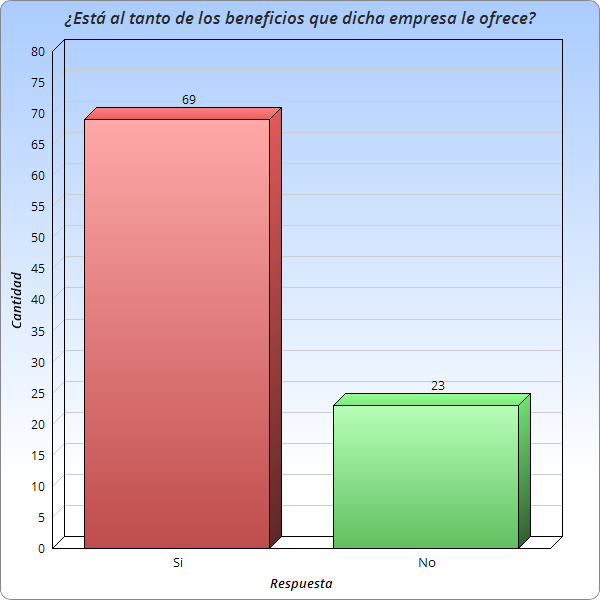
\includegraphics[width=0.6\textwidth]{images/Graficos/graf_5_3.png}
  \caption[chart5.3]{Respuesta a pregunta $5$, conocimiento de beneficios.}
  \label{fig:chart5.3}
  %\url{http://www.chartgo.com/get.do?id=69b1dc7d4e}
\end{figure}

\begin{figure}[!htb]
  \centering
  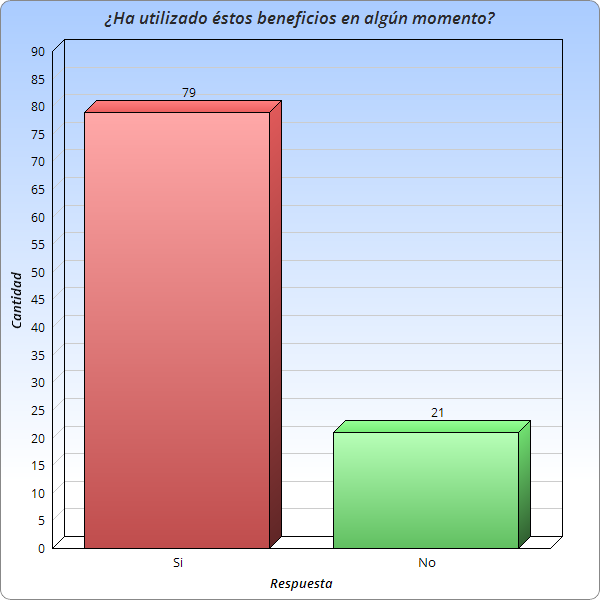
\includegraphics[width=0.6\textwidth]{images/Graficos/graf_5_4.png}
  \caption[chart5.4]{Respuesta a pregunta $6$, utilización de los beneficios.}
  \label{fig:chart5.4}
  %\url{http://www.chartgo.com/get.do?id=69b1dc7d4e}
\end{figure}


La siguiente pregunta, ¿qué beneficios prefiere o preferiría obtener?, tiene como objetivo conocer los
 beneficios mas atractivos para el usuario. Esta pregunta es del tipo \emph{LikeIt}, consta de una
escala de preferencia del $1$ al $5$, $1$ siendo la preferencia menos interesante y 5 la más interesante.
 El beneficio con mas preferencias $5$, o mas interesante para los encuestados, es la obtención de
descuentos en dinero con un $79\%$. El siguiente beneficio con mas interesados es la adquisición
de descuentos para próximas compras con un $32\%$ de los encuestados. Una información importante
obtenida es que una de las herramientas mas utilizadas, obtención de puntos, es resentida por las
personas debido a que existe un mayor rechazo, $22\%$, que aceptación, $18\%$, pero la diferencia
no es sustantiva para descartarla como método a utilizar.
El beneficio mas rechazado, mayor cantidad de $1$, fue la obtención de un reconocimiento por tabla
 de posiciones con un $81\%$.


\begin{figure}[!htb]
  \centering
  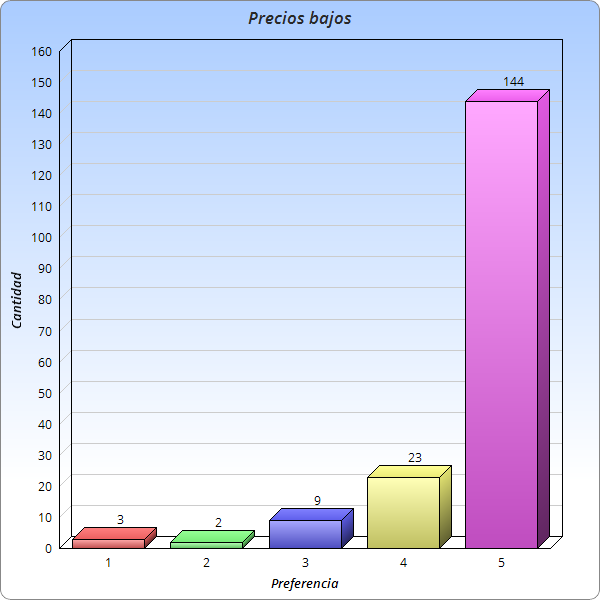
\includegraphics[width=0.6\textwidth]{images/Graficos/graf_5_5.png}
  \caption[chart5.5]{Respuesta a pregunta $7$, cantidad de preferencias a beneficio de precios bajos.}
  \label{fig:chart5.5}
  %\url{http://www.chartgo.com/get.do?id=69b1dc7d4e}
\end{figure}

\begin{figure}[!htb]
  \centering
  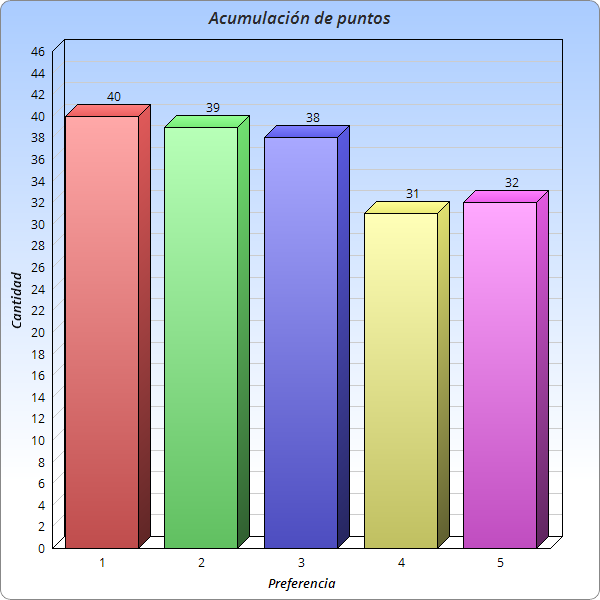
\includegraphics[width=0.6\textwidth]{images/Graficos/graf_5_6.png}
  \caption[chart5.6]{Respuesta a pregunta $7$, cantidad de preferencias a beneficio de acumulación de puntos.}
  \label{fig:chart5.6}
  %\url{http://www.chartgo.com/get.do?id=69b1dc7d4e}
\end{figure}

\begin{figure}[!htb]
  \centering
  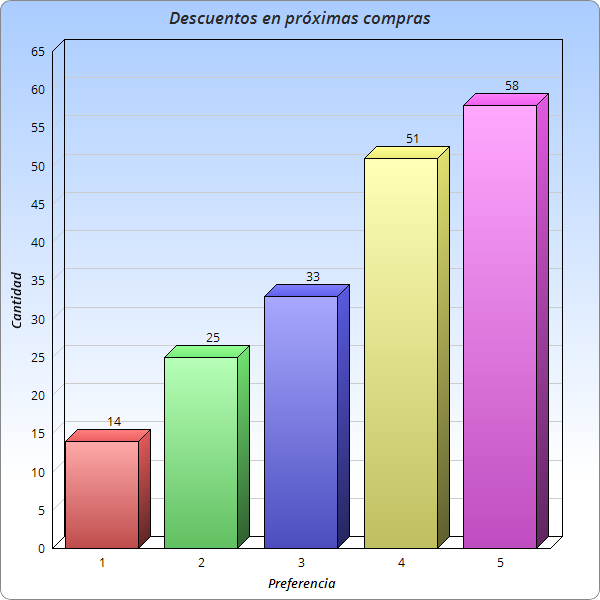
\includegraphics[width=0.6\textwidth]{images/Graficos/graf_5_7.png}
  \caption[chart5.7]{Respuesta a pregunta $7$, cantidad de preferencias a beneficio de descuento en
próximas compras.}
  \label{fig:chart5.7}
  %\url{http://www.chartgo.com/get.do?id=69b1dc7d4e}
\end{figure}

\begin{figure}[!htb]
  \centering
  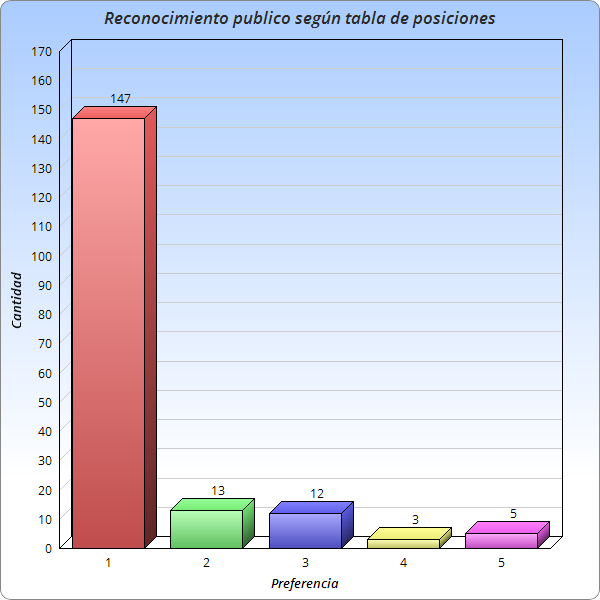
\includegraphics[width=0.6\textwidth]{images/Graficos/graf_5_8.png}
  \caption[chart5.8]{Respuesta a pregunta $7$, cantidad de preferencias a beneficio de reconocimiento
publico según tabla de posiciones.}
  \label{fig:chart5.8}
  %\url{http://www.chartgo.com/get.do?id=69b1dc7d4e}
\end{figure}


La pregunta $8$, ¿cuál es su preferencia a la hora de realizar compras?, muestra cual es la preferencia
a la hora de comprar, presencial u online. La preferencia mas seleccionada, por $134$ personas,
fue la opción de compra presencial. Esto indica que en Chile no se acostumbra a comprar vía internet
y esto representa una oportunidad de negocio debido al incremento de alfabetización digital y
con esto el aumento del acceso al internet.

\begin{figure}[!htb]
  \centering
  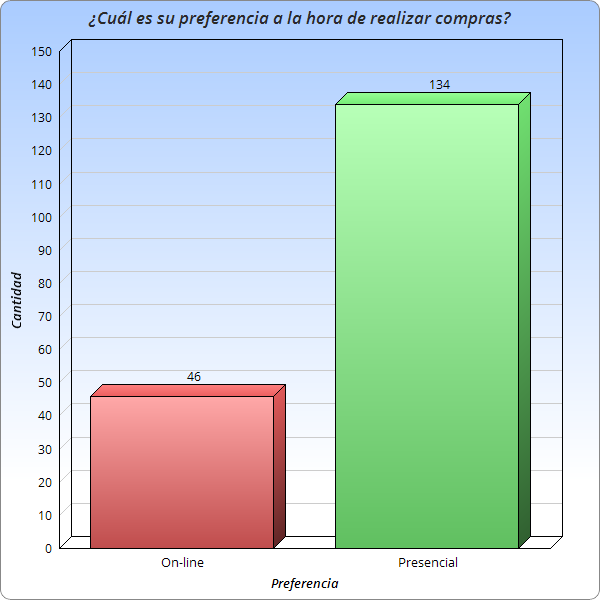
\includegraphics[width=0.6\textwidth]{images/Graficos/graf_5_9.png}
  \caption[chart5.9]{Respuesta a pregunta $8$, preferencia al momento de comprar.}
  \label{fig:chart5.9}
  %\url{http://www.chartgo.com/get.do?id=69b1dc7d4e}
\end{figure}

Una vez respondida la pregunta anterior se le expone al usuario, en la pregunta $9$, si preferiría
utilizar un sitio de ventas online convencional, solo es utilizado para la transacción entre cliente
y empresa, o un sitio el cual le ofrezca herramientas de \emph{gamification}. Con un $69\%$ seleccionan
una tienda con {\GAM} como la alternativa preferida. Con este resultado se remarca la
utilización de este concepto con el fin de atraer a nuevos usuarios.

\begin{figure}[!htb]
  \centering
  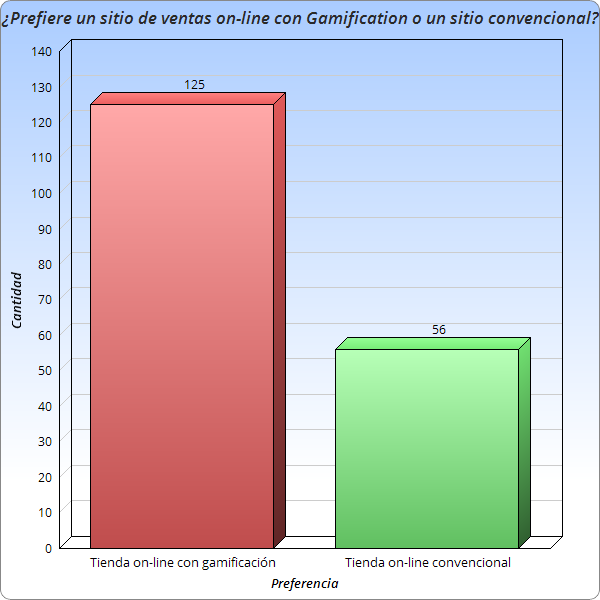
\includegraphics[width=0.6\textwidth]{images/Graficos/graf_5_10.png}
  \caption[chart5.10]{Respuesta a pregunta $9$, preferencia al momento de comprar de forma on-line.}
  \label{fig:chart5.10}
  %\url{http://www.chartgo.com/get.do?id=69b1dc7d4e}
\end{figure}


La pregunta $10$ intenta ratificar una de las mayores ideas tras la utilización de {\GAM},
la motivación. Este sentimiento se crea en el usuario con el fin de atraer y retener a este cliente.
 Se obtuvo que $122$ personas han creado este sentimiento que los impulsa a volver a utilizar o comprar
en la tienda implementada con {\GAM}. Esta información es bastante importante al momento de implementar
una solución gamificada y aun mas cuando se trata de comercio electrónico.

\begin{figure}[!htb]
  \centering
  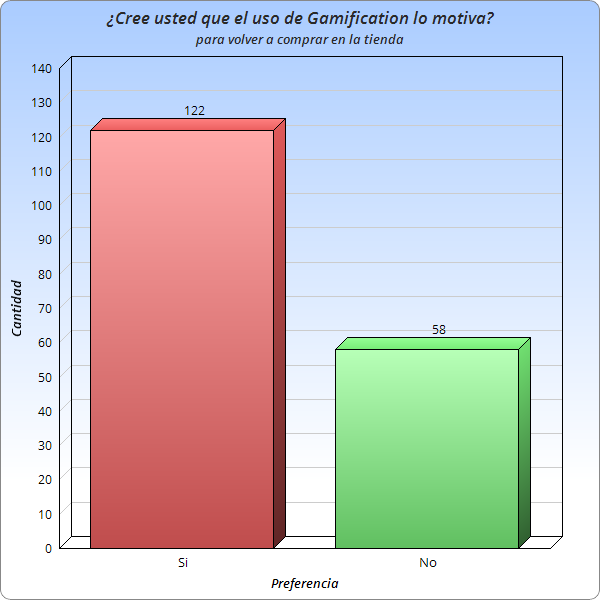
\includegraphics[width=0.6\textwidth]{images/Graficos/graf_5_11.png}
  \caption[chart5.11]{Respuesta a pregunta $10$, motivación para volver a comprar en una misma tienda.}
  \label{fig:chart5.11}
  %\url{http://www.chartgo.com/get.do?id=69b1dc7d4e}
\end{figure}

Por ultimo, se intenta obtener una idea de que contextos podrían ser interesantes para implementar una
solución gamificada. Con esto en mente, la mas votada fue el contexto social con $109$ preferencias,
seguida por educación con $100$ encuestados. Con esta información se pueden inferir ideas para
desarrollos futuros en esta área.

\begin{figure}[!htb]
  \centering
  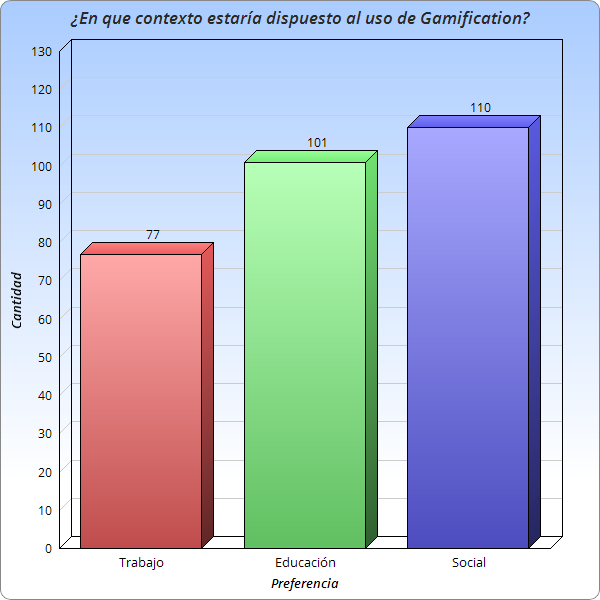
\includegraphics[width=0.6\textwidth]{images/Graficos/graf_5_12.png}
  \caption[chart5.12]{Respuesta a pregunta $11$, contextos a los cuales se le podría implementar {\GAM}.}
  \label{fig:chart5.12}
  %\url{http://www.chartgo.com/get.do?id=69b1dc7d4e}
\end{figure}


Luego de realizar la implementación {\GAM} sobre una tienda online y con los datos obtenidos mediante
la encuesta realizada se obtuvo bastante información para analizar y obtener conclusiones que ayudaran
a futuras empresas que quieran utilizar este concepto en sus empresas. También se obtiene información
para guiar trabajos futuros en otros contextos.
